\subsection{Monte Carlo corrections}

Since the MC samples available show some discrepancies with data we apply weights to lower these discrepancies.
Weighted MC is used thoughout all the process: to get shapes for the fit, to get efficiencies, to train the Neural Networs.
In the following section are described the contribution considered.

\subsubsection{\Bz transverse momentum and number of SPD hits}

First of all, we reweight our MC to match data distributions of \Bz transverse momentum.
To do this we need to compare the \Bz $p_T$ distributions in data and MC.
This cannot be done trivially because the real data events contain background.
Therefore we vfit $\Bz\to\Kstar(\jpsi\to ll)$ events out of stripping and we use it to extract an S-weight.
The S-weight, corresponds to the probability of each event to be signal given its mass.
The fits used to extract the S-weight are reported in Fig.\ref{fig:SweightFit} 

Now combining the real data distribution and the S-weight we obtaine a "clean signal" transverse momentum
distribution which can be compared to the same distribution in MC. We take the ratio of the two
distributions as a weight for the MC. This brings the MC distribution to match the real data one by construction.
The described procedure is done separately for 2011 and 2012 events, for muons and electrons.
In Fig.\ref{fig:B0ptW} is reported the weight in isoposulated bins of \Bz $p_T$ for the electrons and muons channel, for 2011 and 2012 data. 

One other quantity that the MC is known to underestimate is the number of SPD hits important especially
for electron identification. We apply in this case the same procedure used for the \Bz transverse momentum.
In Fig.\ref{fig:SPDW} is reported the weight in isoposulated bins of number of SPD hits for the electrons and muons channels, for 2011 and 2012 data.


\begin{figure}[h!]
\centering
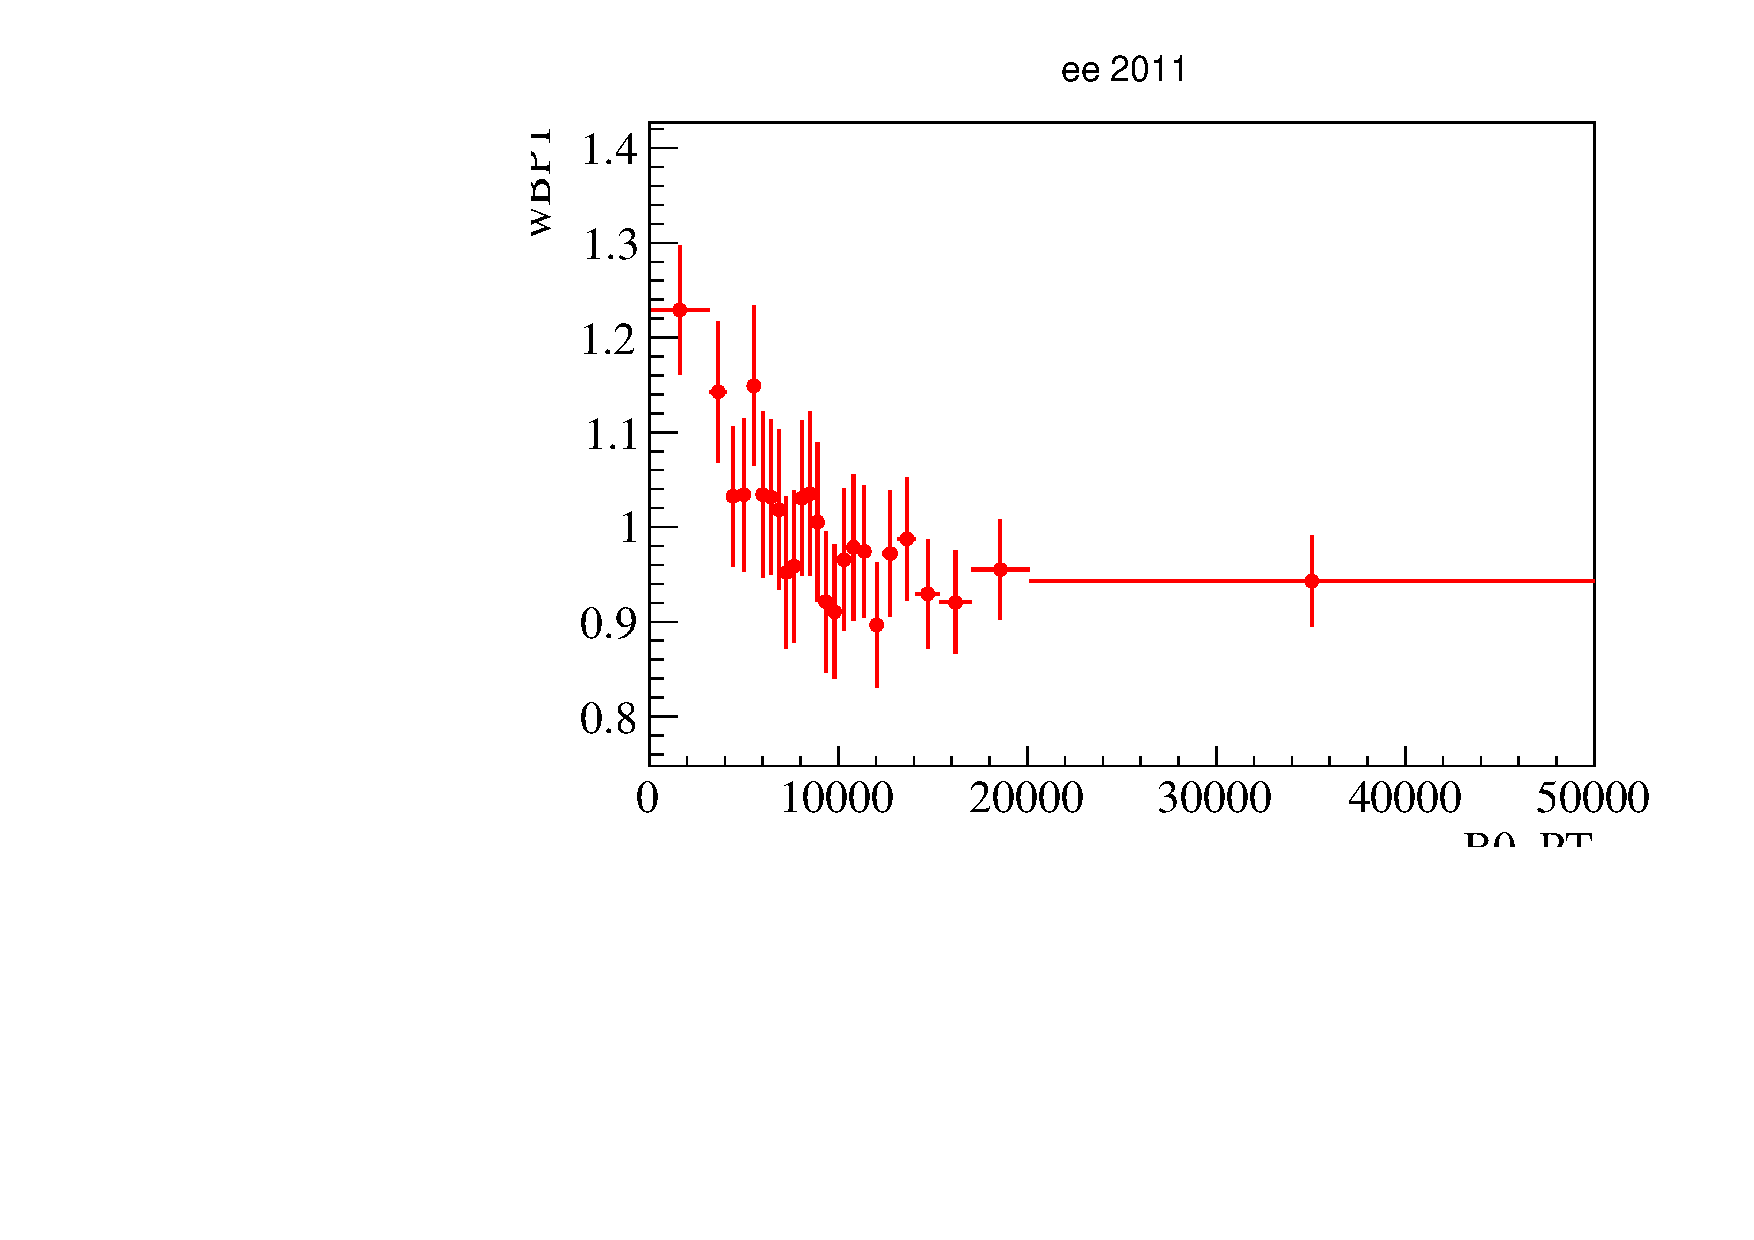
\includegraphics[width=0.40\textwidth]{RKst/figs/Weights/EE_wBPT_2011.pdf}
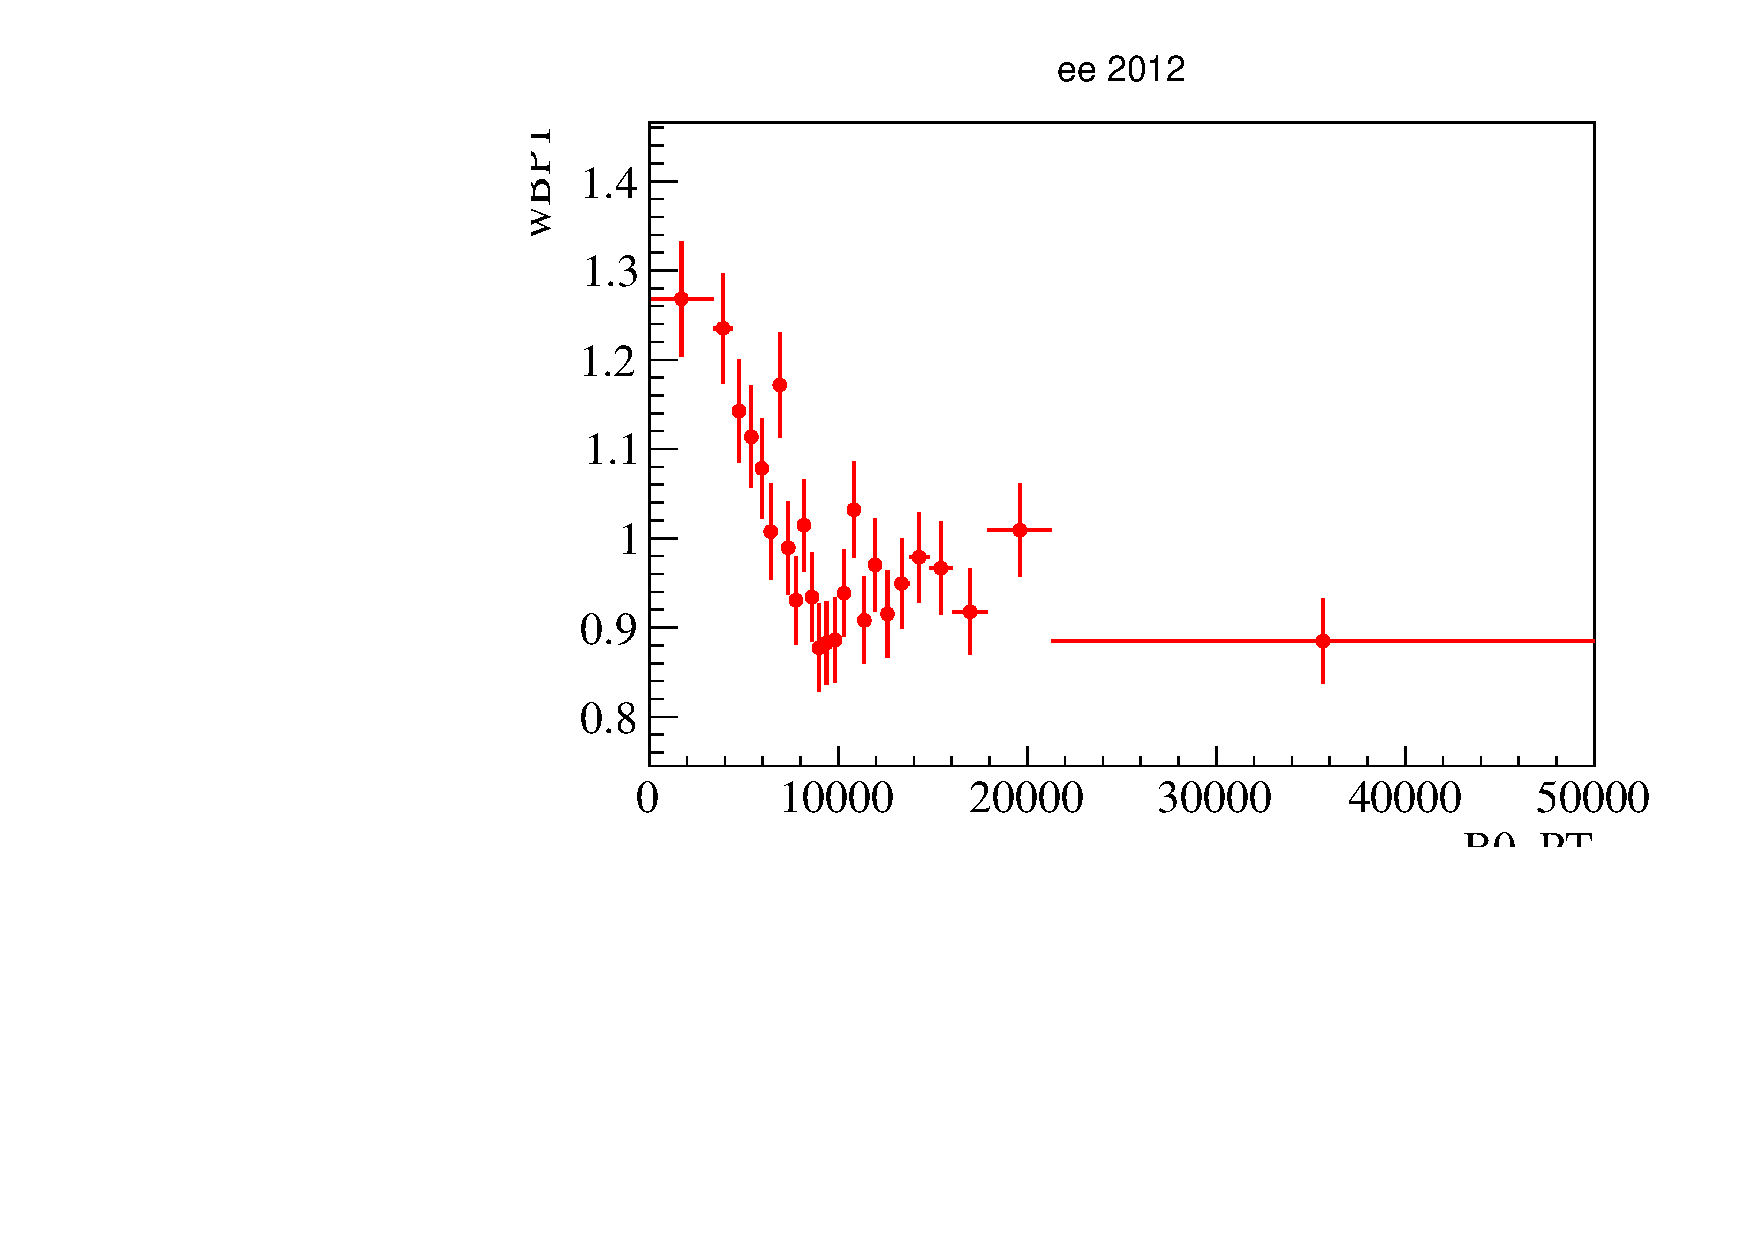
\includegraphics[width=0.40\textwidth]{RKst/figs/Weights/EE_wBPT_2012.pdf} \\
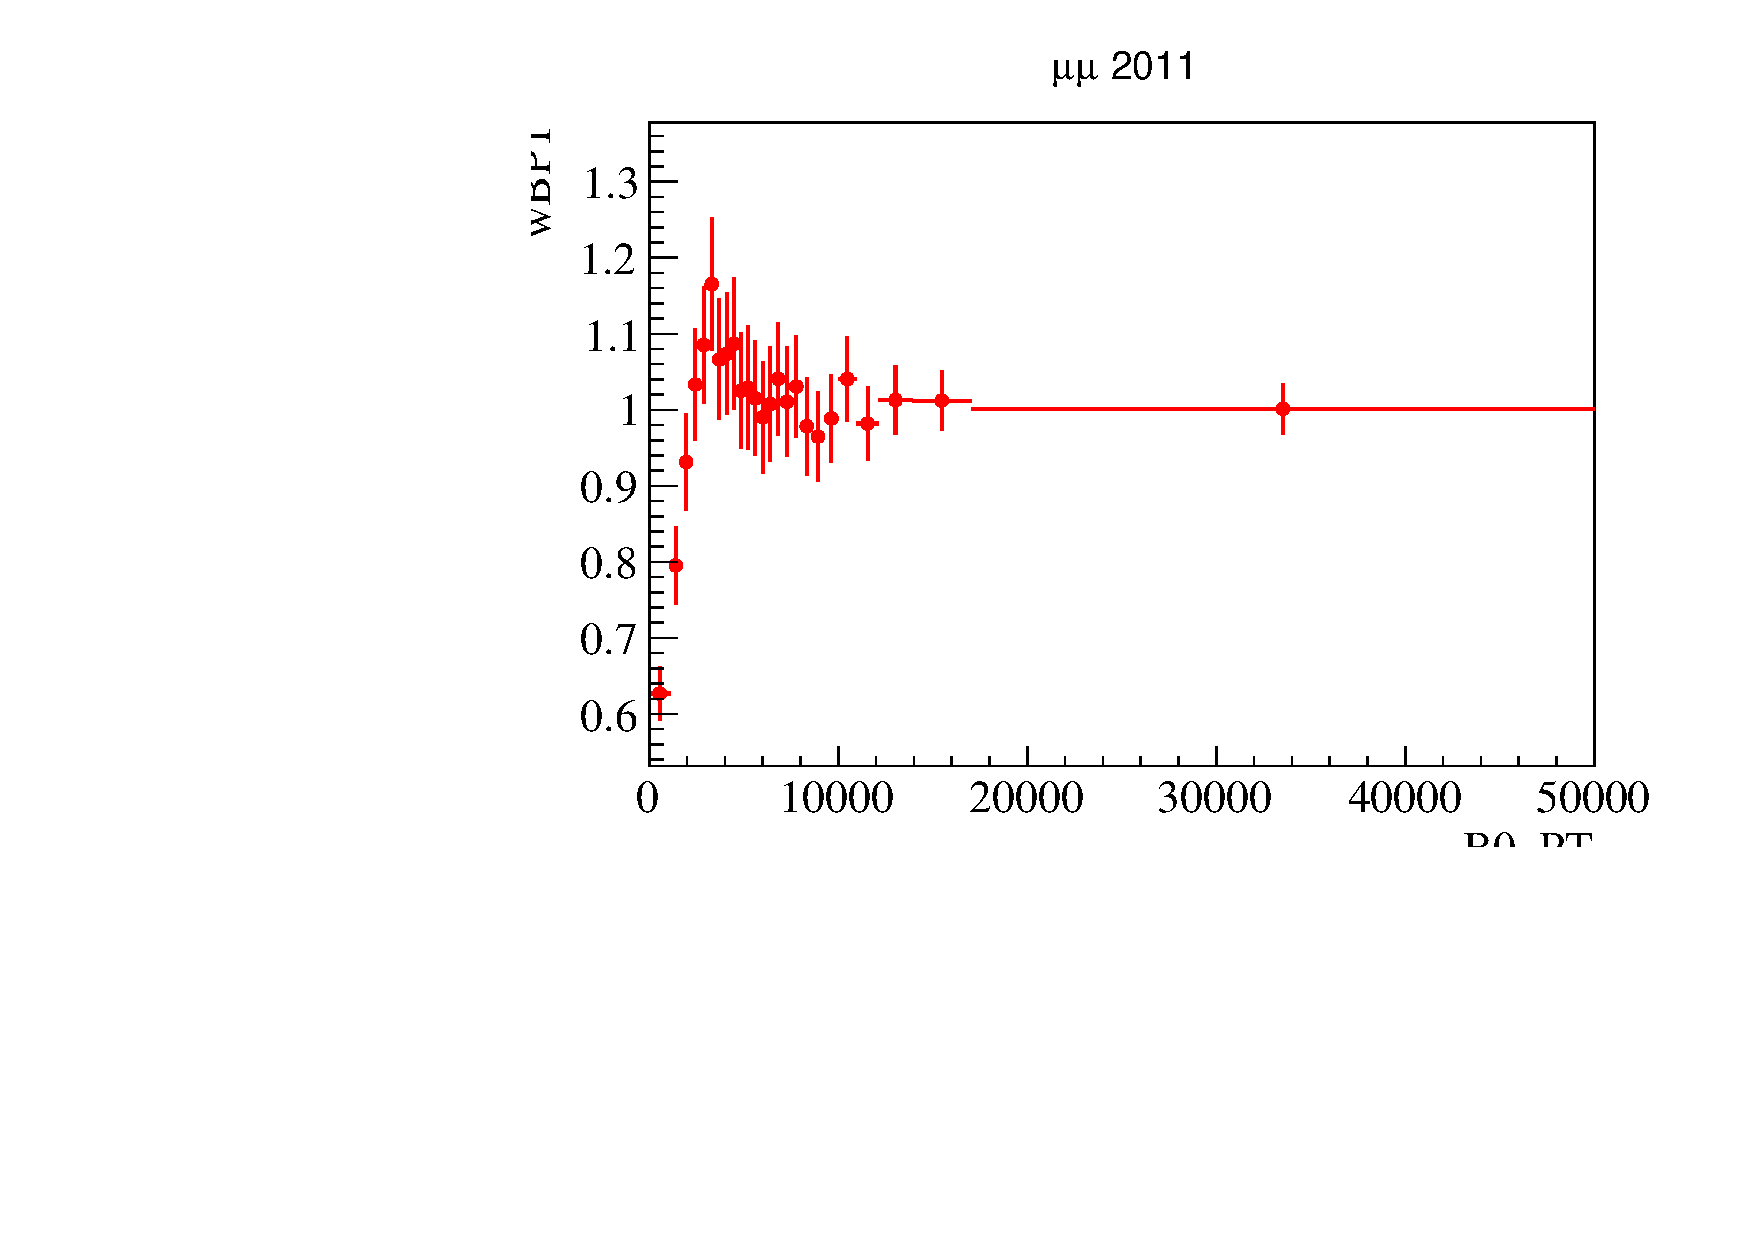
\includegraphics[width=0.40\textwidth]{RKst/figs/Weights/MM_wBPT_2011.pdf}
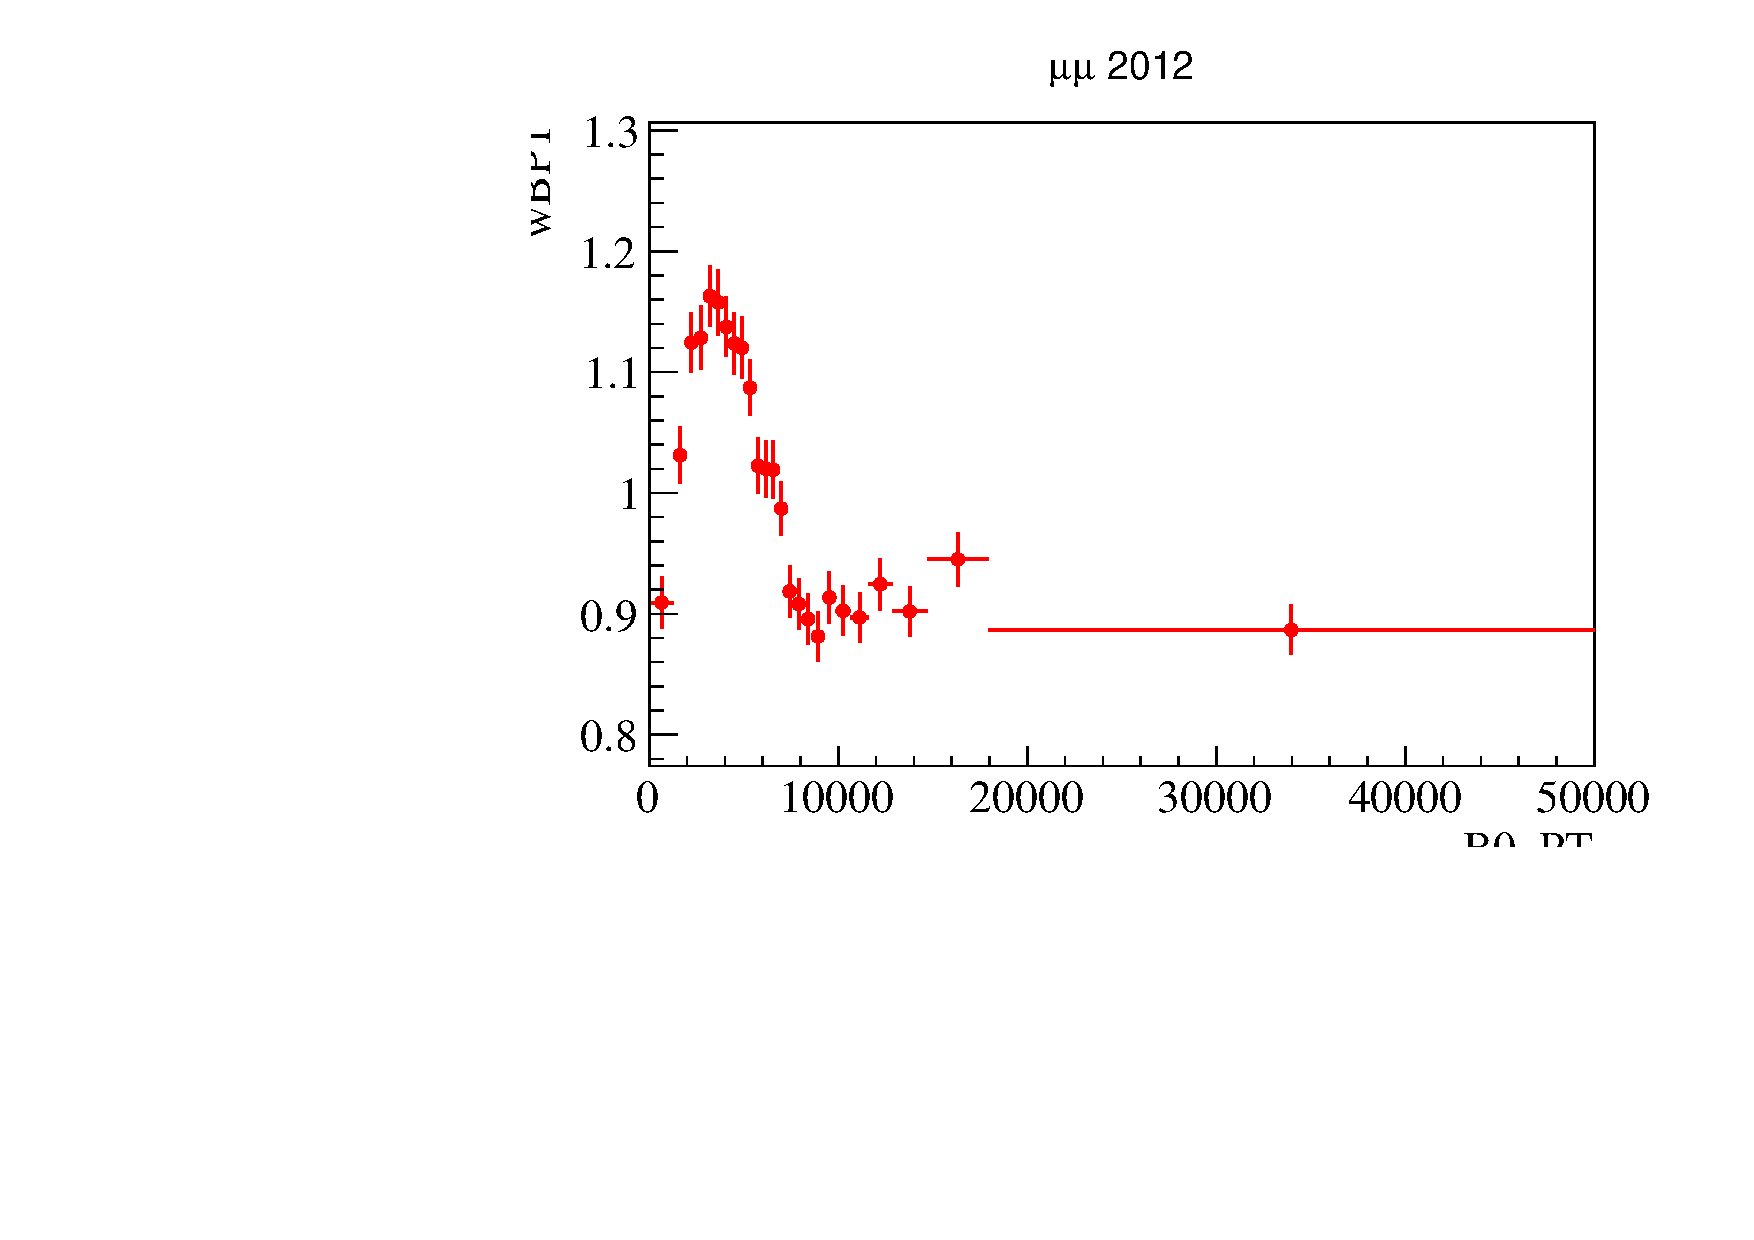
\includegraphics[width=0.40\textwidth]{RKst/figs/Weights/MM_wBPT_2012.pdf}
\caption{Weight applied to MC events in isoposulated bins of \Bz $p_T$ for the electrons (top) and muons (bottom) channel, for 2011 (left) and 2012 (right) data. }
\label{fig:B0ptW}
\end{figure}

\begin{figure}[h!]
\centering
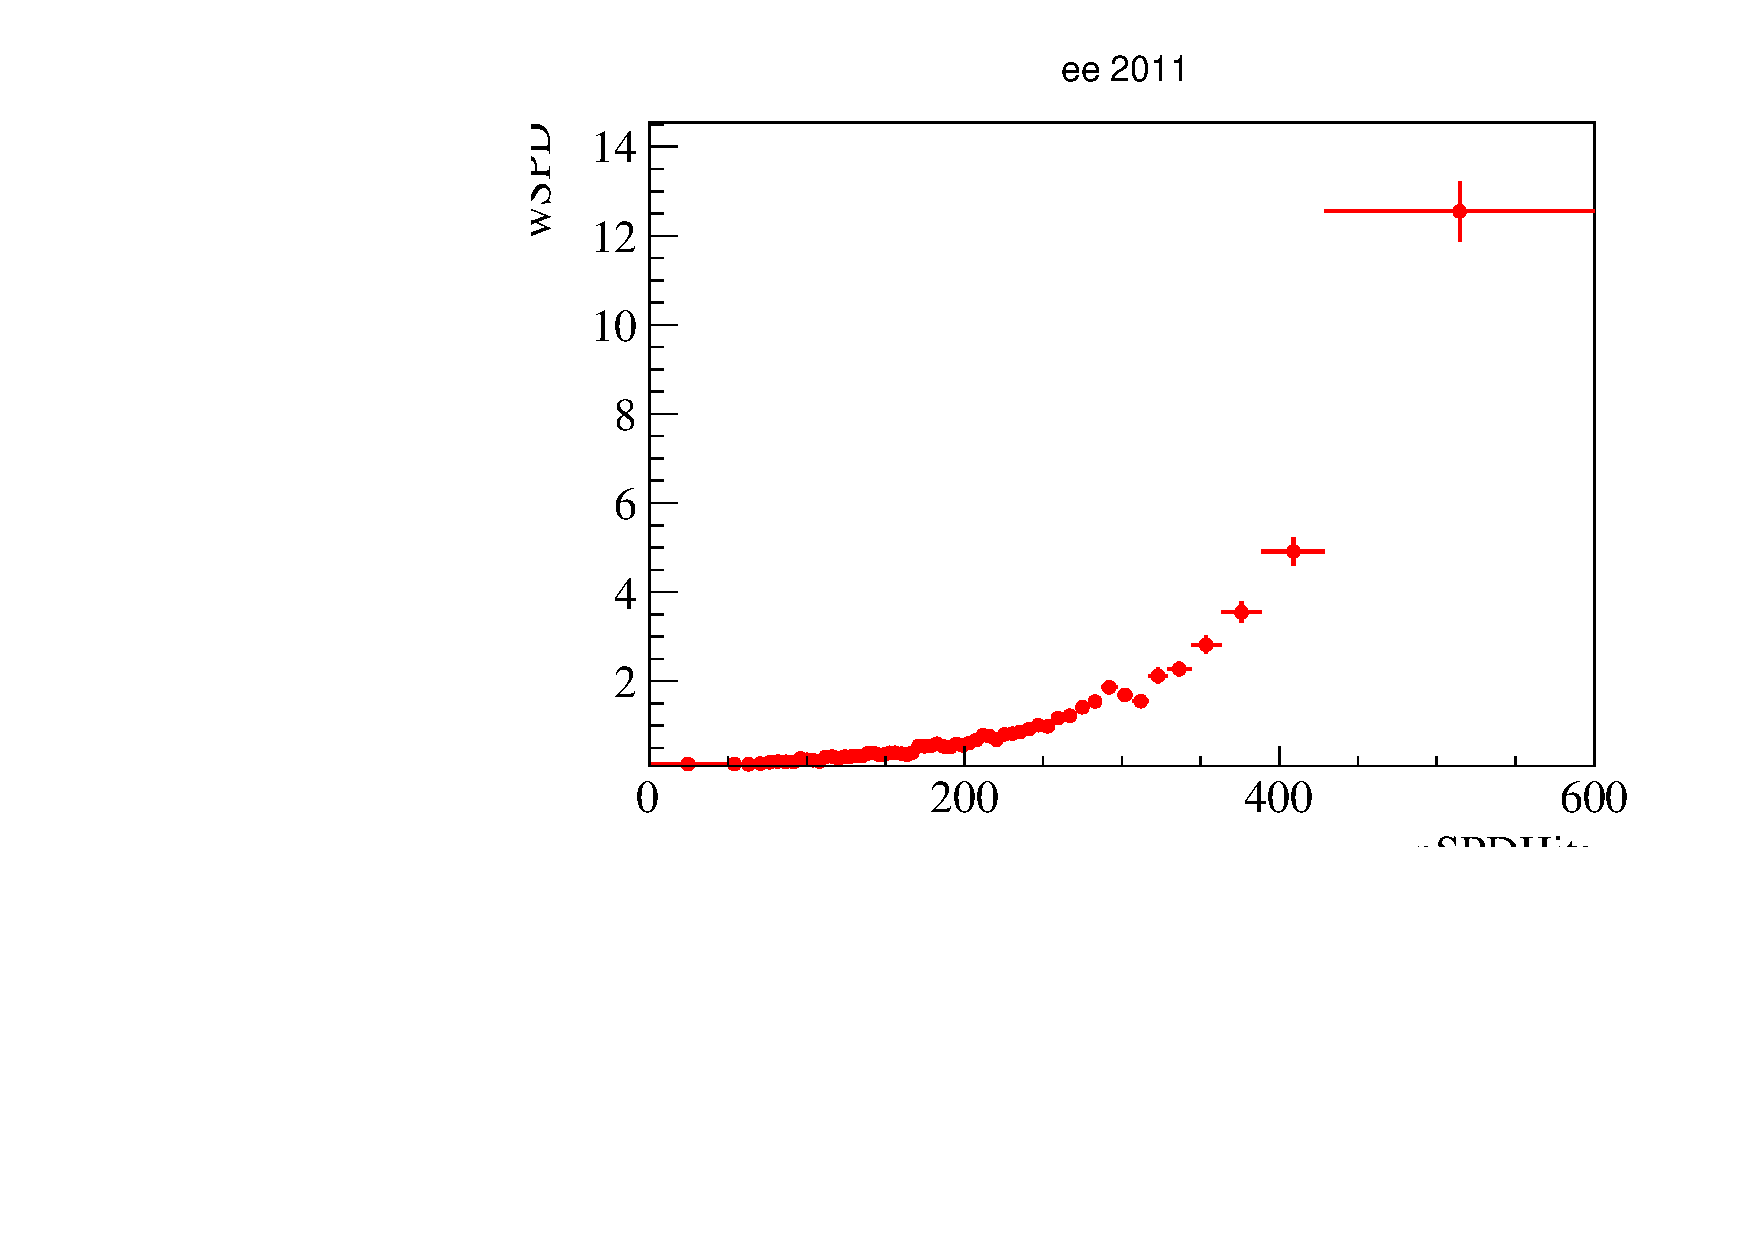
\includegraphics[width=0.40\textwidth]{RKst/figs/Weights/EE_wSPD_2011.pdf}
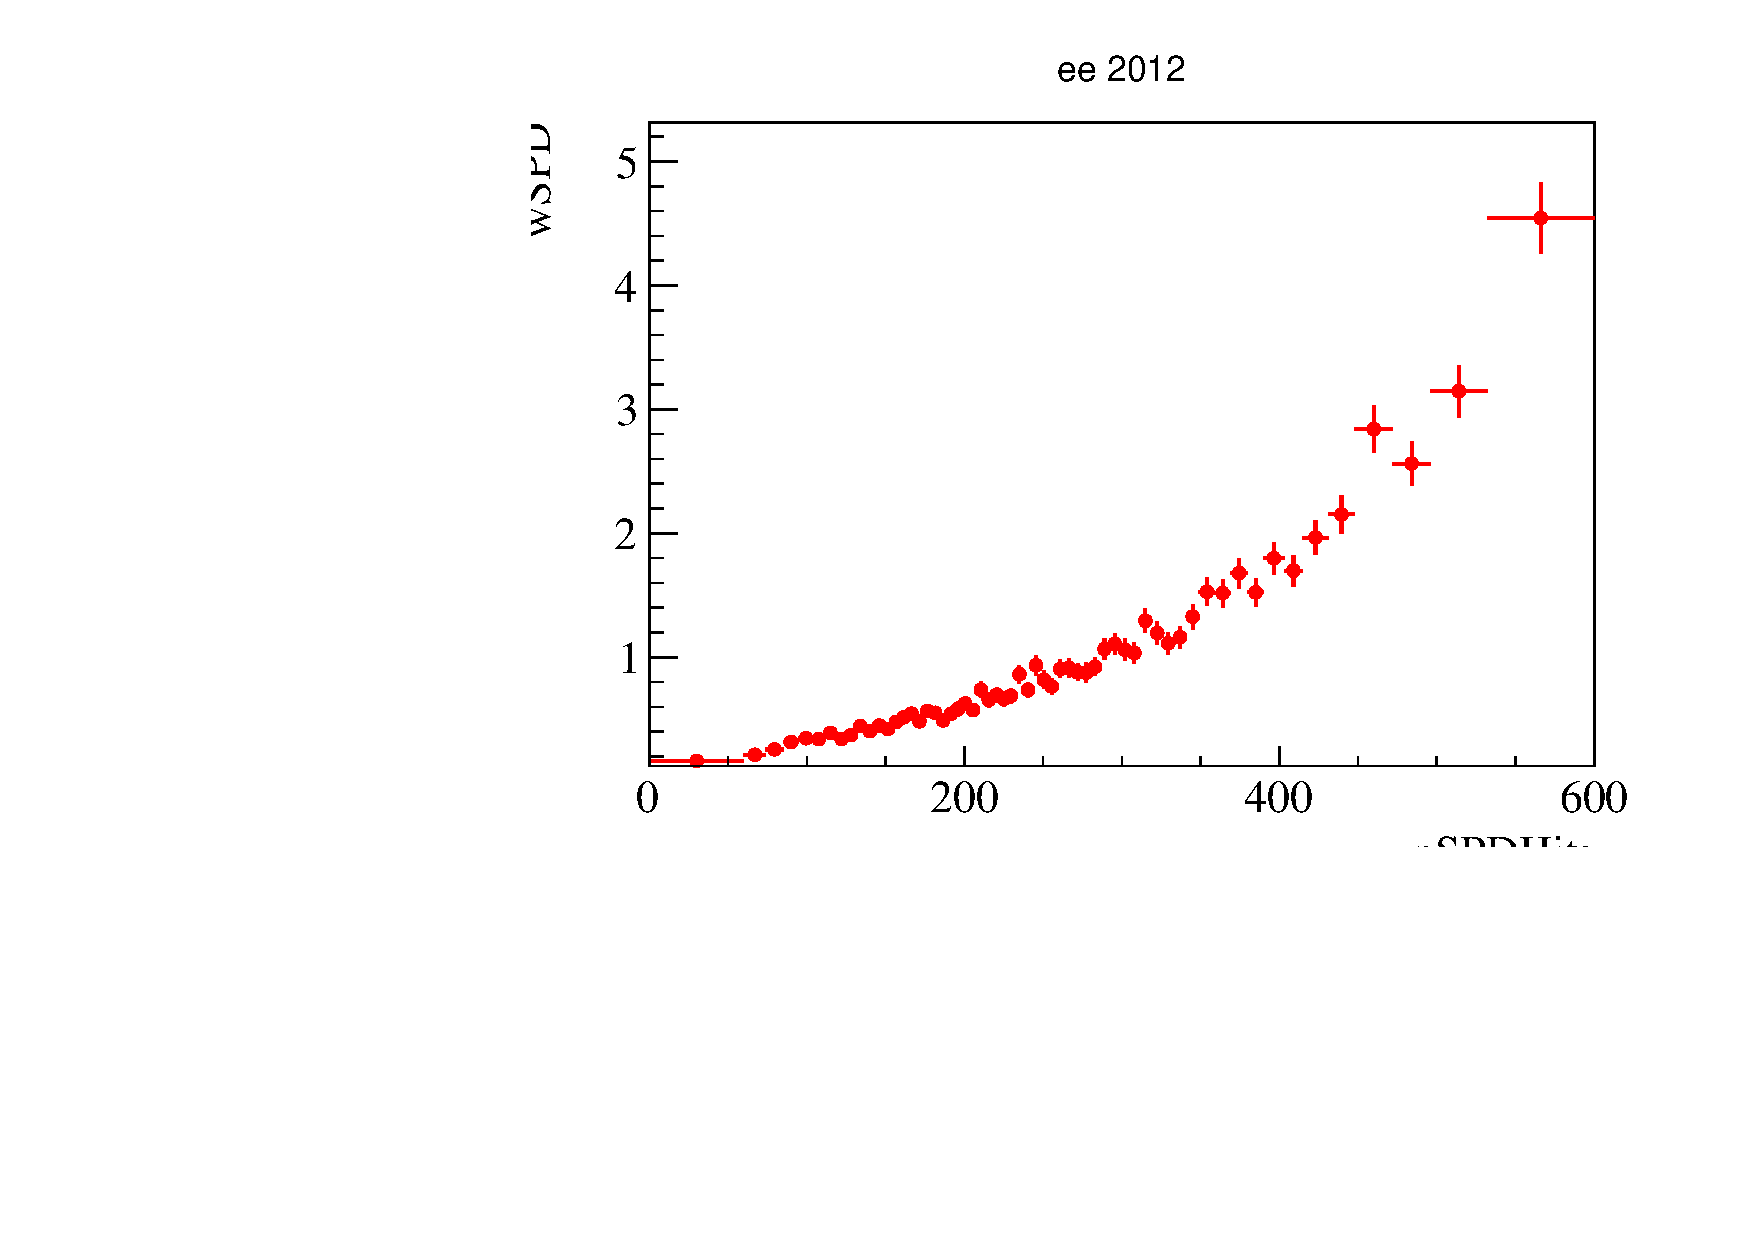
\includegraphics[width=0.40\textwidth]{RKst/figs/Weights/EE_wSPD_2012.pdf} \\
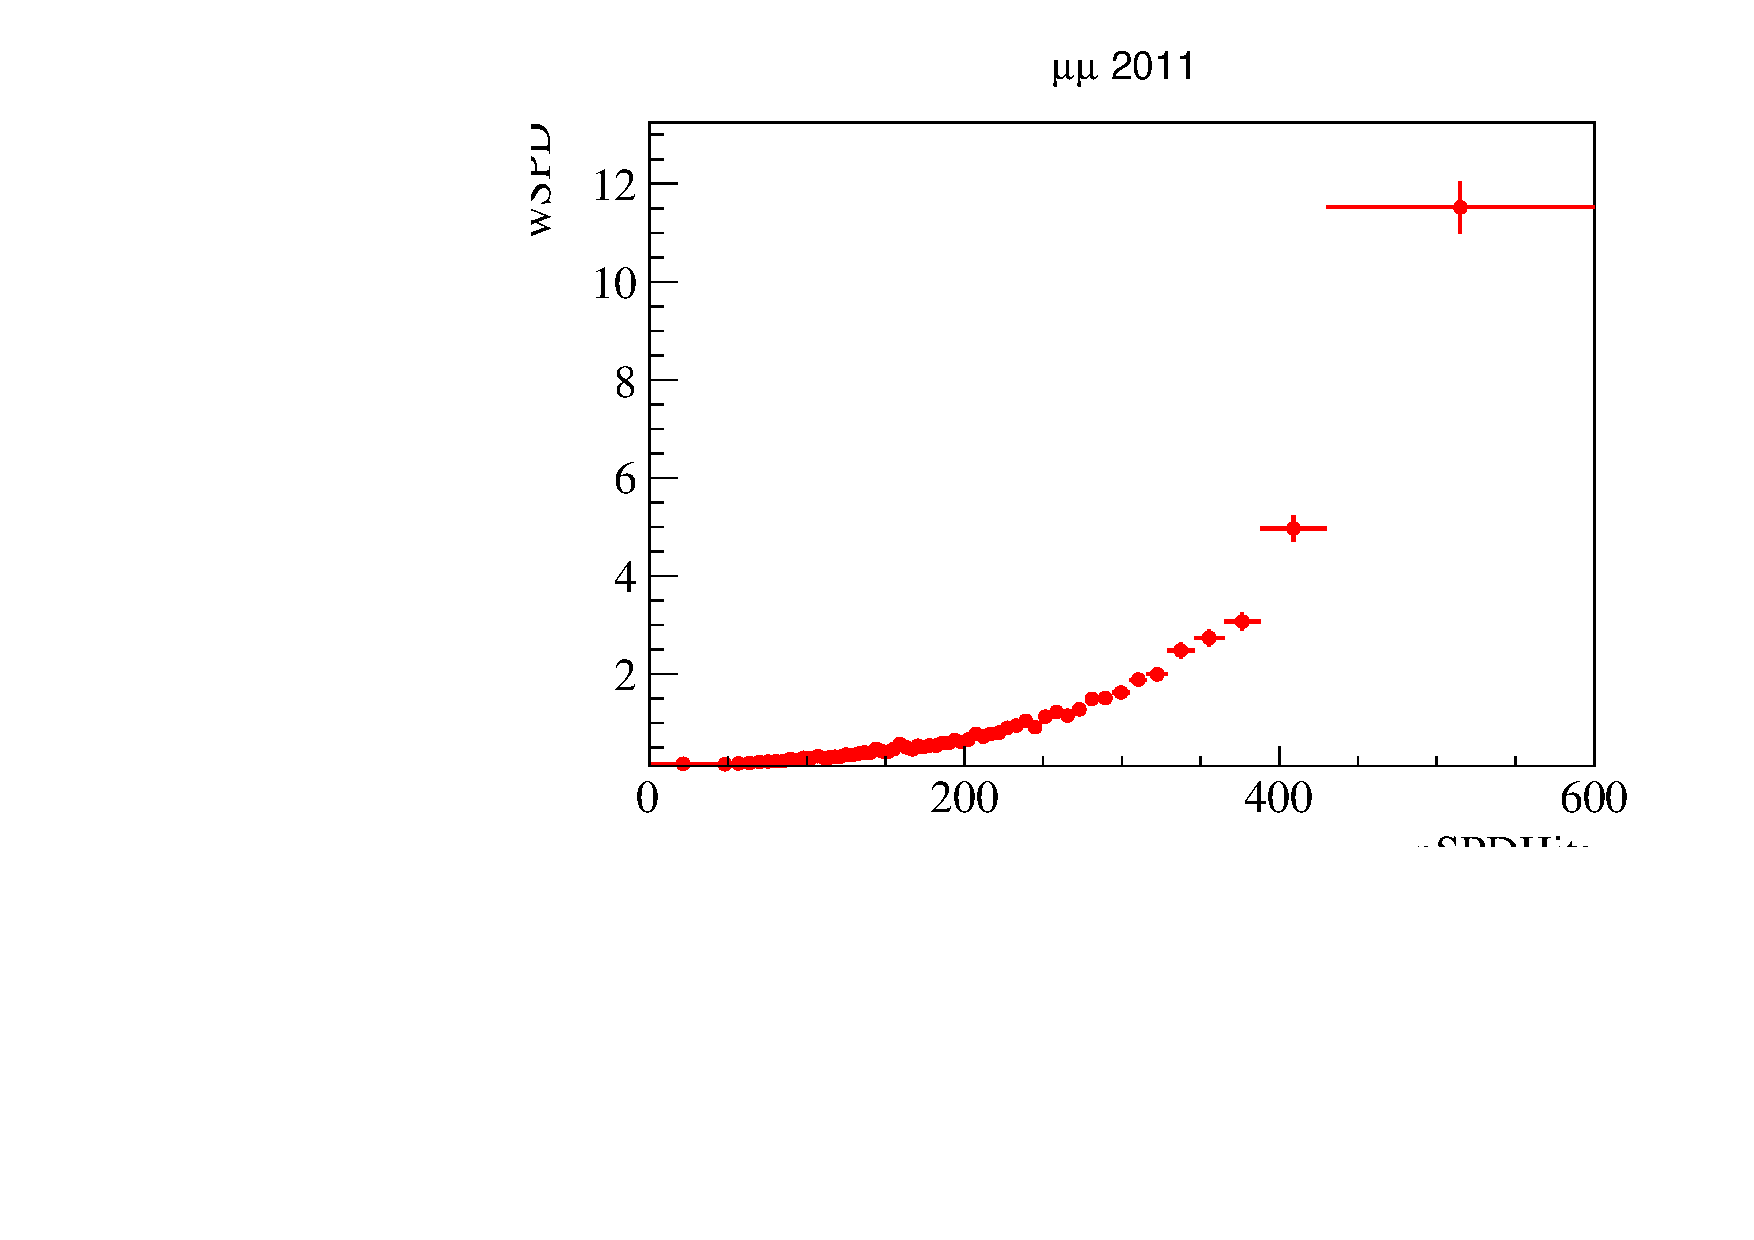
\includegraphics[width=0.40\textwidth]{RKst/figs/Weights/MM_wSPD_2011.pdf}
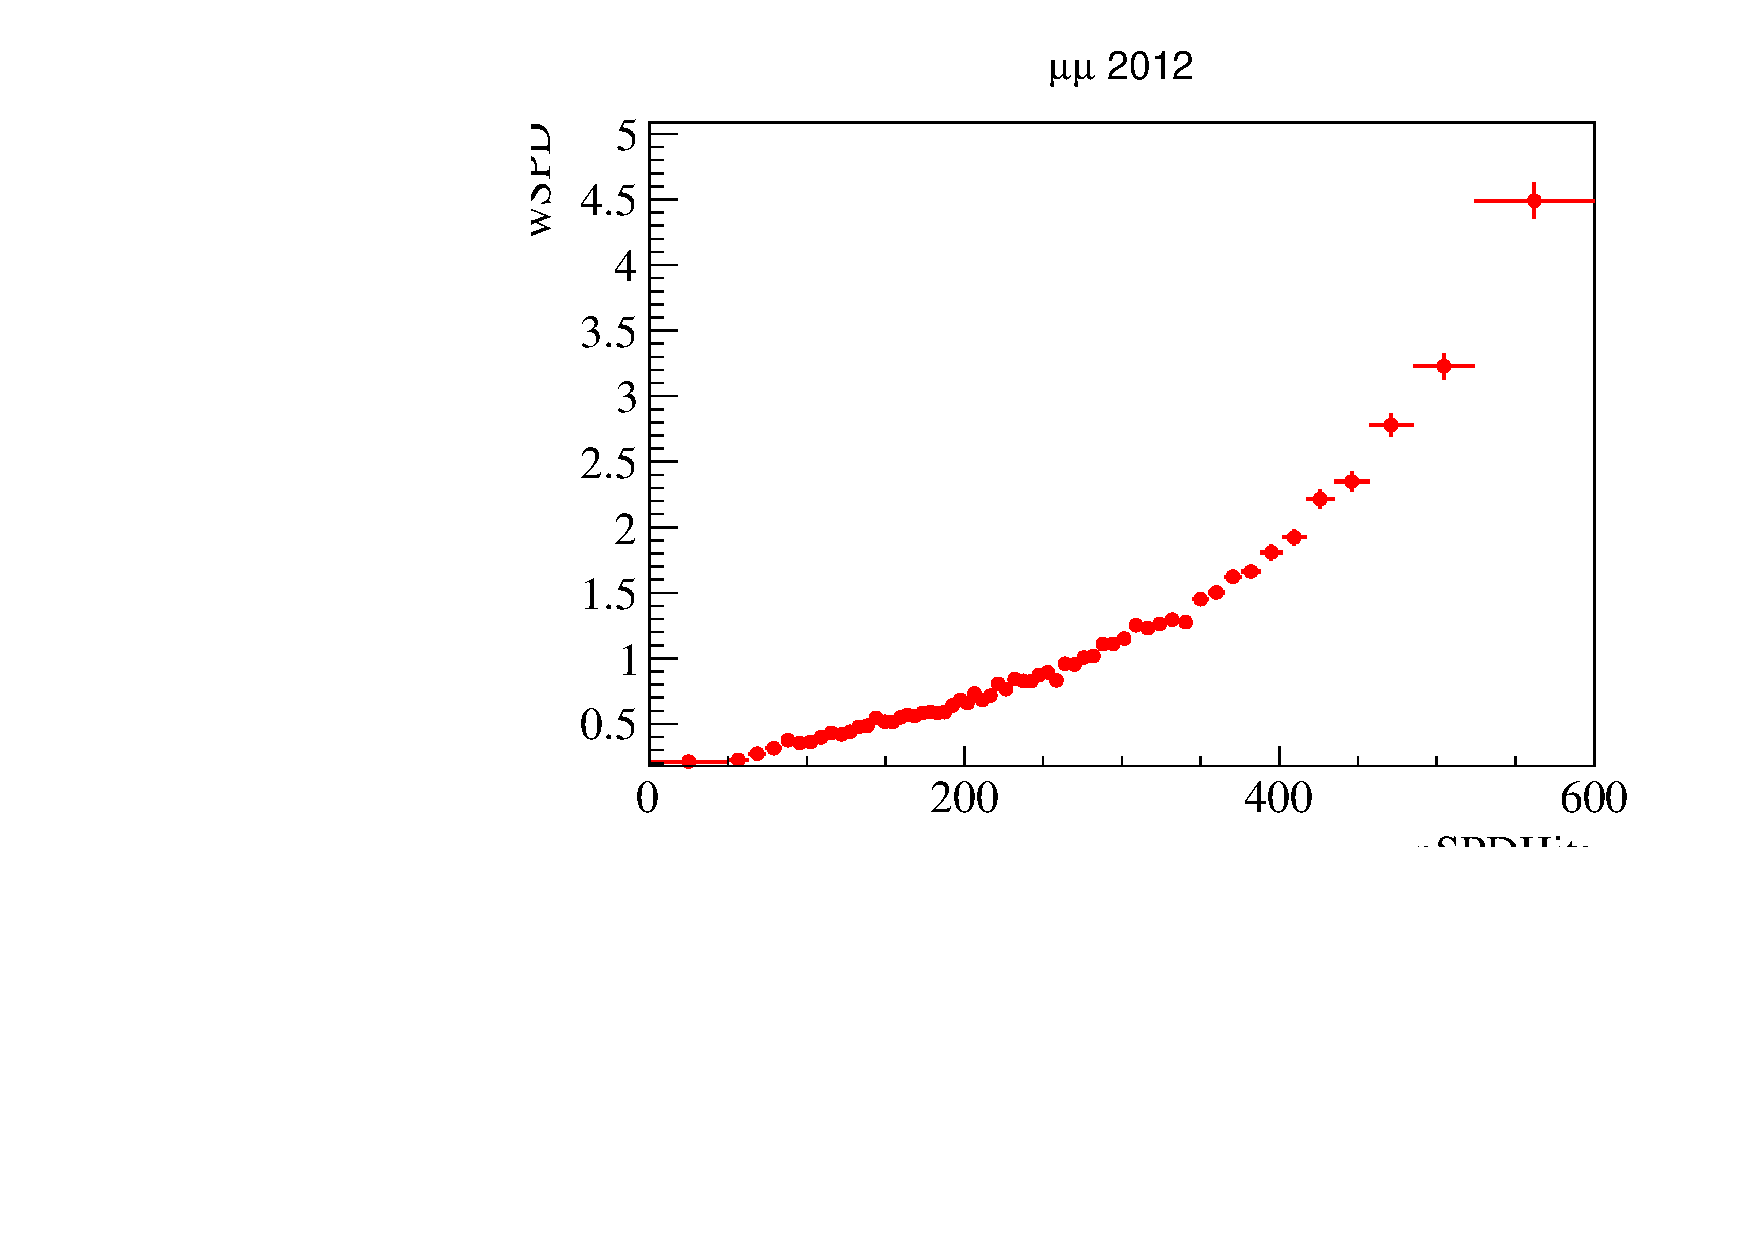
\includegraphics[width=0.40\textwidth]{RKst/figs/Weights/MM_wSPD_2012.pdf}
\caption{Weight applied to MC events in isoposulated bins of number of SPD hits for the electrons (top) and muons (bottom) channel, for 2011 (left) and 2012 (right) data. }
\label{fig:SPDW}
\end{figure}

\subsubsection{PID weighting}

The PID variables are also known not to match between data and MC. For this reason we use a data drive method to find the efficiency as
descibed in \ref{sec:PIDeff}. Nevertheless the MC is used to find shapes to use in the fits and these shapes could be affected
by the differences in the PID variables. For this reason we use the same data driven method to get a table of PID efficiencies
as a function of momentum and pseudorapidity of tracks and we use this to reweight out MC. More details can me found in \ref{sec:PIDeff}.

\subsubsection{Trigger efficiency}

{\em Simone scrivi qualcosa io di sta roba non so nulla}



\clearpage
